% This is the master file of the folder structure.

% First, the preamble needs to be called. This contains all the 'under the hood' stuff for your document.
% Use \input rather than than \include for .tex files, because \input can be nested and don't include a page break.
% This file contains your LaTeX preamble. A preamble is a part of your document where all required packages and macros can be defined. This needs to be done before the \begin{document} command.

% Documentclass:
% Standard LaTeX classes are: article, book, report, slides, and letter. These cover the basis, but are not best. More advanced users might want to try out the KOMA classes or the memoir class. Optional arguments: 10pt. The font size of the main content is set to 10pt with the option between [].
\documentclass{llncs}
\usepackage[utf8]{inputenc}

% Geometry:
% The papersize of the document is defined with the geometry package. Here, the size is set to A4 with a4paper. Other possibilities are a5paper, b5paper, letterpaper, legalpaper and executivepaper.
\usepackage[a4paper]{geometry}

% AMS math packages:
% Required for proper math display.
%\usepackage{amsmath,amsfonts,amsthm}	% conflict with the llncs package
\usepackage{amsmath,amsfonts}			% to avoid conflict with the llncs package
%\usepackage{amsfont} create a conflict so it's not used
\usepackage{amssymb}
\usepackage{mathtools}
% For case equation with nested label
% \usepackage{cases} NOT USEFUL



% Graphicx:
% If you want to include graphics in your document, the graphicx package is required.
\usepackage{graphicx}

% Graphic path declaration:
\graphicspath{{figs/}}

% Tabu:
% To test if this package could be the latest package for my work
\usepackage{tabu}

% [OLD] Booktabs:
% The booktabs package is needed for better looking tables. 
\usepackage{booktabs}

% [OLD] Tables:
\usepackage[table]{xcolor}
\usepackage{multirow}
%\usepackage{tabularx}

\newcommand{\win}{\cellcolor[gray]{0.9}}

% Enumeration:
% To manipulate the listing of object
\usepackage[inline]{enumitem}
\setlist*[enumerate,1]{%
	label=(\roman*),
}
% [Alternative]
%\usepackage{easylist}

% SIunitx:
% The SIunitx package enables the \SI{}{} command. It provides an easy way of working with (SI) units.
\usepackage{siunitx}

% URL:
% Clickable URL's can be made with this package: \url{}.
%\usepackage{url}

% Caption:
% For better looking captions. See caption documentation on how to change the format of the captions.
%\usepackage{caption}

% Hyperref:
% This package makes all references within your document clickable. By default, these references will become boxed and colored. This is turned back to normal with the \hypersetup command below.
\usepackage{hyperref}
\hypersetup{colorlinks=false,pdfborder=0 0 0}

% Cleveref:
% This package automatically detects the type of reference (equation, table, etc.) when the \cref{} command is used. It then adds a word in front of the reference, i.e. Fig. in front of a reference to a figure. With the \crefname{}{}{} command, these words may be changed.
\usepackage{cleveref}
\crefname{equation}{equation}{equations}
\crefname{figure}{figure}{figures}	
\crefname{table}{table}{tables}

% Pseudo code packages:
\usepackage[ruled,linesnumbered]{algorithm2e}
\usepackage{algorithmicx}
\usepackage{algpseudocode}

% Verbatim:
% Typewriter formatting and comment environment
\usepackage{verbatim}

% Bibliography style
%\usepackage{natbib}



% Command

% For the level structure depending of the 

% The title page is created with the command \maketitle which needs to be placed after the \begin{document} command. To create the titlepage, some entries are needed: the name of the autor is defined by \author{}, the title by the entry \title{} and the date by the command \date{}. Note that the current date is displayed with \today.

\author{Luca Ambrosini\inst{1} \and Giancarlo Nicol\`{o}\inst{2}}
\title{Comparative study of neural models for the COSET shared task at IberEval 2017}
\date{}

%\titlerunning{<Your abbreviated contribution title>}
%\authorrunning{<abbreviated author list>}
\institute{Scuola Universitaria Professionale della Svizzera Italiana
\and Univesitat Polit\`{e}cnica De Val\`{e}ncia\\
\email{luca.ambrosini@supsi.ch\\ giani1@inf.upv.es}}




% All the actual content of your document should be placed after \begin{document} and before \end{document}. This content should be placed in the docs folder and can then be called with \input{docs/filename}.
\begin{document}

% Here the actual title page is printed, based on the given entries \author{}, \title{} and \date{}.
\maketitle

% The table of contents can be automatically generated with the \tableofcontents command. Note that you need to compile the document twice in order to see the changes in the table of contents.
%\tableofcontents

% List of figures
%\listoffigures
 
% List of tables
%\listoftables

% The list of algorithm
%\listofalgorithms

% The \input{} command reads and processes the indicated example.tex file. Note that docs/ locates the folder where the .tex file is stored.
\abstract

Version one

This paper describes an explorative approach to create from scratch a set of baselines for tackling tweet classification problems using natural language processing and machine learning techniques.
Our approach focuses on neural network models taken from state of the art that exploit different corpus preprocessing, tweets representations and features extraction methods.
Finally, we will discuss how we applied this methodology to the \emph{Classification Of Spanish Election Tweets (COSET)} task at IberEval 2017 and present the results we obtained

Version two

This paper describes our participation in the \emph{Classification Of Spanish Election Tweets (COSET)} task at IberEval 2017.
During the searching process for the best classification system to send for the competition, we developed a comparative study over possible combination of corpus preprocessing, text representations and classification models. After an initial models exploration, we focus our attention over specific neural models.
Interesting insight can be drawn from the comparative study helping future practitioner tackling tweets classification problems to create system baseline for their work.

Possible add for the report in general and 

handcrafted features

explain that we haven't put a proper module for handcrafted features, but our modular approach to solve the classification problem lead to an easy customization and integration of a proper module for these handcrafted features.		% Abstract
\section{Introduction} \label{sec:introduction}

Intro over nlp and text classification: motivation why this field is important and the actual challenge and open problems (will be top just to list some problem and their way to be solved, for example citing the different workshop that we had during the course)


Text classification is an important task in Natural Language Processing with many applications, such as web search, information retrieval, ranking and document classification (Deerwester et al., 1990; Pang and Lee, 2008). Recently, models based on neural networks have become increasingly popular (Kim, 2014; Zhang and LeCun, 2015; Conneau et al., 2016). While these models achieve very good performance in practice, they tend to be relatively slow both at train and test time, limiting their use on very large datasets.

The 

vedi citazioni su word embedding di mark e bag of word da maite

Introduce informally our task and list some way of tackling this problem from the different perspectives, maybe say that we de-construct tthe actual approach and cathegorized their inner process in: representation, preprocessing, model and post processing (that we haven't done).

Finally explain how we structured this report

In the following we firstly describe the 

In this paper we describe our participation for addressing
the PR-SOCO task. The rest of the paper is organized as
follows. Next section is devoted to dene the Personality
Recognition task. In Section 4 the model proposed is described.
Following, in Section 5, the results achieved are
presented. Finally, in Section 6 our results are discussed,
and future work is proposed.


	% Introduction
\section{Task definition} \label{sec:task}

The COSET shared task's aim was to classify Spanish written tweets talking about the 2015 Spanish General Election, where each tweet had to be classified into one of five different categories:
\begin{enumerate*}
\item political issues, related to the most abstract electoral confrontation; 
\item policy issues, about sectorial policies; 
\item personal issues, on the life and activities of the candidates; 
\item campaign issues, related with the evolution of the campaign;
\item and other issues.
\end{enumerate*}

Participants had access to a labelled corpus composed of training set (2242 tweets) and development set (250 tweets) for system benchmarking. We analysed it and find the following statistical information that guided us in the baselines building:
\begin{multicols}{2}
\begin{itemize}
	\item Average train sequence length:
	\begin{itemize}
		\item 135 chars 
		\item 24 words
	\end{itemize}
	\item Max train sequence length: 
	\begin{itemize}
		\item 140 chars
		\item 49 words
	\end{itemize}
\end{itemize}
\end{multicols}			% Task description
\section{Systems description} \label{sec:system}

In this section we describe the tweet classification systems we built. From a module perspective we can describe our systems as composed of three main blocks: text pre-preprocessing (\Cref{subsec:preprocessing}),  text representation (\Cref{subsec:representation}) and classification model (\Cref{subsec:classificationModel}). 


\subsection{Initial investigation} \label{subsec:boh}
To address the tweets classification problem we began our investigation analysing some of the most widely used text representations and classifiers.
In the analysing for possible text representations we began focusing our attention on lexical features based on: \emph{Bag Of Words} \cite{harris1954distributional},\emph{Bag Of N-Grams} (bigrams and trigrams), both with and without \emph{term frequency-inverse document frequency} normalization (i.e., TF-IDF norm).
In relation to classification models that can exploit the above representations,  we analysed \emph{Random Forest, Decision Trees, Support Vector Machines} and \emph{Multi Layer Perceptron}. Since the results obtained with the combination of those \emph{model + representation} were outperformed by neural network based models, we decided not to report their analysis in this paper, but rather focus on the module description of the neural models.


\subsection{Text pre-processing} \label{subsec:preprocessing}
Regarding the text pre-preprocessing, has to be mentioned that the corpus under observation can not be treated as proper written language, because computer-mediated communication (CMC) is highly informal, affecting diamesic\footnote{The variation in a language across medium of communication (e.g. Spanish over the phone versus Spanish over email)} variation with creation of new items supposed to pertain lexicon and graphematic domains \cite{bazzanella2011oscillazioni,cerruti2013netspeak}.
Therefore, in addition to well know pre-processing approach, as stemming (i.e., ST), stopwords (i.e., SW) and punctuation removal (i.e., PR), specific tweets pre-processing techniques has to be taken in consideration.

From previous consideration, we define a set of specific tweet pre-processing approach that take into consideration the following items:
\begin{enumerate*}
\item mentions (i.e., MT),
\item smiley (i.e., SM),
\item emoji (i.e., EM),
\item hashtags (i.e., HT),
\item numbers (i.e., NUM),
\item URL (i.e., URL)
\item and Tweeter reserve-word as RT and FAV (i.e., RW).
\end{enumerate*}

For each of these items we left the possibility to be removed or substituted by constant string (e.g.
\begin{enumerate*}
\item \emph{Pre-processing of @Ambros and \#atoppe :)} $\xrightarrow{substitution} $ \emph{Pre-processing of \$MENTION and \$HASHTAG \$SMILEY},
\item \emph{Pre-processing of @Ambros and \#atoppe :)} $\xrightarrow{removing} $ \emph{Pre-processing of and}
\end{enumerate*}
).

To implement above pre-processing tecnique we took advantage of the following tools:
\begin{enumerate*}
\item NLTK \cite{nltk} and 
\item Preprocessor\footnote{Preprocessor is a preprocessing library for tweet data written in Python, https://github.com/s/preprocessor}.
\end{enumerate*}



\subsection{Text representation} \label{subsec:representation}
The use of neural model suggest us to exploit recent trend over text representation, in particular we decided to use embedding vectors as representation following the approach described by \cite{bojanowski2016enriching}, where tweet elements like \emph{words} and \emph{word n-grams} are represented as vectors of real number with fixed dimension $|v|$.
In this way a whole sentence $s$, with length $|s|$ its number of word, is represented as a \emph{sentence-matrix} $M$ of dimension $|M| = |s| \times |v|$. $|M|$ has to be fixed a priori, therefore $|s|$ and $|v|$ have to be estimated. $|v|$ was fixed to 300 following \cite{bojanowski2016enriching}. $|s|$ was left as a system parameter that after optimization (via grid search) was fixed to $|s| = 30$, with this choice 
input sentences longer than $|s|$ are truncated, while shorter ones are padded with null vectors (i.e., a vector of all zeros).
Depending of chosen tweets elements a different embedding function has to be estimated (i.e., learnt), in the continuation we are going to analyse the possible choices.

\subsubsection{Word embedding.}
Choosing words as elements to be mapped by the embedding function, raise some challenge over the function estimation related to data availability. In our case the available corpus is very small and estimated embeddings could lead to low performance.
To solve this problem, we decided to use a pre-trained embeddings estimated over Wikipedia using a particular approach called \emph{fastText} \cite{bojanowski2016enriching}, this choice was made after previous tries over other embeddings estimated from other corpus that lead to poor performance.

Using this approach, after the sentence-matrix embeddings are calculated, following \cite{bojanowski2016enriching} terminologies, matrix's weights can be set to \emph{static} or \emph{non-static}. In the latter case, backward propagation will be able to adjust its values otherwise they will stay fixed as initially calculated by the embedding function.

In this way four possible combination of sentence-matrix embeddings can be formulated: 
\begin{enumerate*}
\item the use of a pre-trained embedding function (i.e., FastText from Wikipedia) and
\item static or non-static weights.
\end{enumerate*}
From this combination the one composed of static weight without pre-trained embeddings won't be take in consideration for obvious reasons, meaning that the cases in consideration will be three:
\begin{enumerate*}
	\item ES static,
	\item ES non-static,
	\item (no pre-trained embeddings) non-static.
\end{enumerate*}

\begin{comment}
From this combination the one composed of static weight without pre-trained embeddings won't be take in consideration for obvious reasons, while we decided to use two pre-trained function from Spanish (i.e., ES) and Catalan (i.e., CA) to see how the use of pre-trained embeddings of a similar language will perform in relation to static/non-static weights.
Meaning that the cases in consideration will be five:
\begin{enumerate*}
\item ES static,
\item CA static,
\item ES non-static,
\item CA non-static,
\item (no pre-trained embeddings) non-static.
\end{enumerate*}
\end{comment}

\subsubsection{N-gram embedding.}
Choosing n-grams as element to be mapped by the embedding function, raises more challenges respect simple words, because no pre-trained embeddings are available and in this case the corpus has to be significantly big, otherwise n-gram frequencies will be really low and the estimation algorithm is not able to learn a valid embedding.
Our insight was empirically validated by a very low performance. Nevertheless, as explained in the following, this embedding will be used in a particular model that won't rely its performance just over n-gram embeddings.


\subsection{Classification models} \label{subsec:classificationModel}
Following, we describe the neural models used for the classification module, where for each of them the input layer uses text representations described in \Cref{subsec:representation} (i.e., sentence-matrix).


\subsubsection{Fast text.}
This model was introduced in \cite{joulin2016bag}, where its main difference from our neural model is the use of a particular input layer. In details, rather than using only words or only n-gram as element for the embedding, both elements are embedded with the aim of capturing partial information about words order.
The architecture's idea  is illustrated in \Cref{fig:fastText}.Here the input layer is directly fed into a \emph{Global Average Pooling} layer, that transforms the sentence-matrix in a single vector, that is projected into two dense layers.
Regarding the architectural references in \cite{joulin2016bag}, they used a number of hidden layers fixed to ten, but we measured better performance using just two layers, moreover we integrate both dropout, gaussian noise and batch normalization.

\begin{figure}[h]
\footnotesize
\centering
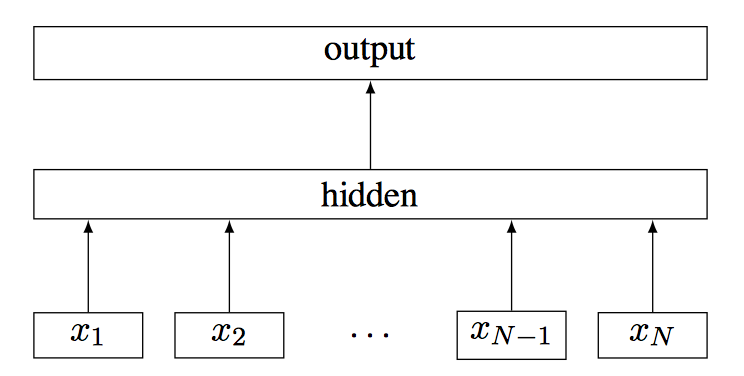
\includegraphics[width=.5\columnwidth]{fast_text}
\caption{Model architecture of \emph{fastText} for a sentence with $N$ n-gram features $x_1,\dots,x_N$. The features are embedded and averaged to form the hidden variable \cite{joulin2016bag}.}
\label{fig:fastText}
\end{figure}


\subsubsection{Convolutional Neural Network.}
Convolutional Neural Networks (CNN) are considered state of the art in many text classification problem. Therefore, we decide to use them in a simple architecture composed by a convolutional layer, followed by a \emph{Global Max Pooling} layer and two dense layers.
Between the two dense layers we used dropout(0.2) to avoid overfitting.

\subsubsection{KIM.}
This model was introduced in \cite{kim2014convolutional}. It can be seen as a particular CNN where the convolutional layer has multiple kernels' size and feature maps.
The complete architecture is illustrated in \Cref{fig:kim}, here the input layer (i.e., sentence-matrix) is processed in a convolutional layer of multiple filters with different sizes, each of these results are fed into \emph{Max Pooling} layers and finally the concatenation of them (previously flatten to be dimensional coherent) is projected into a dense layer.
The intuition behind this model is that smaller filter should be able to capture short sentence patterns similar to n-grams, while bigger ones should capture sentence level features.
Regarding the architectural references in \cite{kim2014convolutional}, the number filter $|f|$ and their size was optimized (via grid search) leading to the following results: $|f| = 4, f_1 = 2\times2, f_2 = 3\times3, f_3 = 5\times5, f_4 = 7\times7$.

\begin{figure}[h]
\footnotesize
\centering
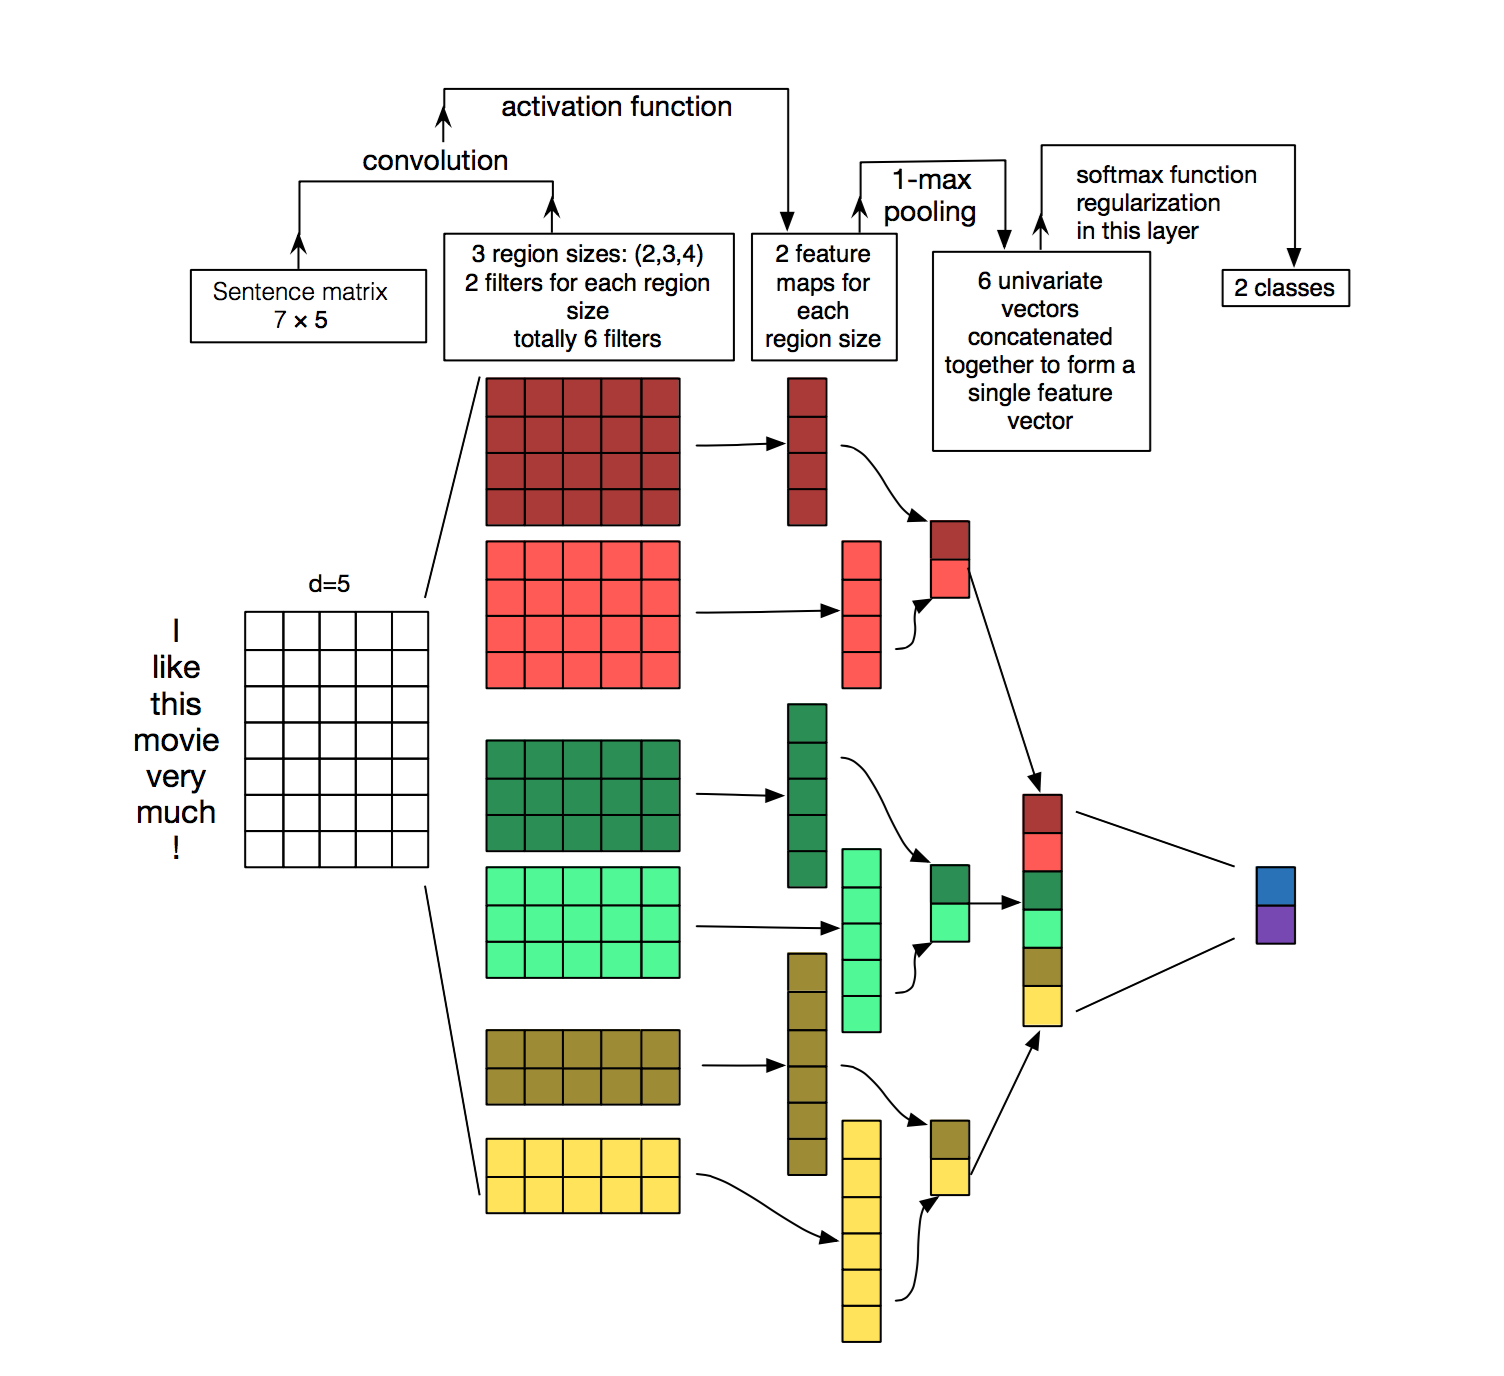
\includegraphics[width=.75\columnwidth]{kim_cnn}
\caption{Illustration of a Convolutional Neural Network (CNN) architecture for sentence classification \cite{zhang2015sensitivity}.}
\label{fig:kim}
\end{figure}

\subsubsection{Long short-term memory.}
LSTM is a type of Recurrent Neural Network (RNN) that is relatively insensitive to gap length. Thanks to this behaviour, they are considered state of the art in some NLP problems.
Our architecture was made of an embedded input layer followed by an LSTM layer of 128 units, terminated by a dense layer. Moreover, to avoid overfitting we used dropout (0.25) and recurrent dropout (0.25).

\subsubsection{Bidirectional LSTM.} Similar to the previous model, bidirectional LSTM is a variation of LSTM where the two RNN receive different inputs, the original and its reverse order, and their results are connected through the recurrent layers.
Our architecture follow the previous one with an LSTM layer of 128 units terminating with two dense layers, where all layers used dropout (0.25) and recurrent dropout(0.25).

		% Methods description
\section{Evaluation} \label{sec:evaluation}

\subsection{Metrics}

\begin{equation}
F_{1-macro} = \frac{1}{|L|} \displaystyle\sum_{l\in L} F_1(y_l, \hat{y}_l)
\end{equation}

\begin{equation}
F_1 = 2 \cdot \frac{precision \cdot recall }{precision + recall}
\end{equation}

\begin{equation}
precision = \frac{1}{|L|} \displaystyle\sum_{l\in L} Pr(y_l, \hat{y}_l)
\end{equation}

\begin{equation}
recall = \frac{1}{|L|} \displaystyle\sum_{l\in L} R(y_l, \hat{y}_l)
\end{equation}


\subsection{Results}

Put an intro over the results that will be analyzed and then comments over them

table of only the 5 models main models and 6 kind of preprocessing
only the mean and say that is 10 fold CV

table of word representation




		% Methods evaluations
\section{Conclusions} \label{sec:conclusion}

In this paper we have presented our participation in the IberEval2017 Classification Of Spanish Election Tweets (COSET) shared task. Five different neural models were explored, in combination with 11 types of preprocessing. No preprocessing emerged to be the best with every kind of model, indicating that the preprocessing pipeline optimization has a big impact on results.
We also explored static vs non-static word embeddings and non-static vectors initialized with pre-trained vectors on a bigger corpus is the best performing combination.


	% Conclusions



% The bibliography is printed with \bibliography{}. With the command \bibliographystyle{} a style is picked.
%\bibliographystyle{plain} 		% for [1] cite style
%\bibliographystyle{plainnat}	% for [Surname et al] cite style
\bibliographystyle{splncs}		% FOR LNCS
%\bibliography{refs/references}
\begin{thebibliography}{1}

\bibitem{kim2014convolutional}
Kim, Yoon. "Convolutional neural networks for sentence classification." arXiv preprint arXiv:1408.5882 (2014).

\bibitem{joulin2016bag}
Joulin, Armand, et al. "Bag of tricks for efficient text classification." arXiv preprint arXiv:1607.01759 (2016).

\bibitem{nltk}
Edward Loper and Steven Bird. 2002. NLTK: the Natural Language Toolkit. In Proceedings of the ACL-02 Workshop on Effective tools and methodologies for teaching natural language processing and computational linguistics - Volume 1 (ETMTNLP '02), Vol. 1. Association for Computational Linguistics, Stroudsburg, PA, USA, 63-70. DOI=http://dx.doi.org/10.3115/1118108.1118117

\bibitem{tweets-preprocessor}
Preprocessor is a preprocessing library for tweet data written in Python, https://github.com/s/preprocessor
\end{thebibliography}	% Conclusions

% To close your document, add the \end{document} command. Everything after this command will not be processed.
\end{document}